\lab{Applications}{Image Compression (SVD)}{SVD}

\objective{Explore the SVD as a method of image compression}

The singular value decomposition is very useful.  In this lab, we are going to explore how the SVD can be used to compress image data.  Recall that the SVD is a decomposition of an $m \times n$ matrix $A$
of rank $r$ into the product $A = U \Sigma V^H$, where $U$ and $V$
are unitary matrices having dimensions $m \times m$ and $n \times n$,
respectively, and $\Sigma$ is an $m \times n$ diagonal matrix
\begin{equation*}
\Sigma = \mbox{diag}(\sigma_1,\sigma_2,\ldots,\sigma_r,0,\ldots,0)
\end{equation*}
where $\sigma_1 \geq \sigma_2 \geq \ldots \geq \sigma_r > 0$ are the
singular values of $A$.  Upon closer inspection, we can write
\begin{equation*}
U = \begin{pmatrix}U_1 & U_2\end{pmatrix}, \quad \Sigma =
\begin{pmatrix}\Sigma_r & 0\\0 & 0\end{pmatrix}, \quad V =
\begin{pmatrix}V_1 & V_2\end{pmatrix},
\end{equation*}
where $U_1$ and $V_1$ have dimensions $m\times r$ and $n\times r$
respectively and $\Sigma_r$ is the $r\times r$ diagonal matrix of
(nonzero) singular values.  Multiplying this out yields the reduced
form of the SVD
\begin{equation*}
A =
\begin{pmatrix}U_1 & U_2\end{pmatrix}
\begin{pmatrix}\Sigma_r & 0\\0 & 0\end{pmatrix}
\begin{pmatrix}V^H_1 \\ V^H_2\end{pmatrix} =
U_1 \Sigma_r V_1^H
\end{equation*}

\subsection*{Low rank data storage}
If the rank of a given matrix is significantly smaller than its
dimensions, the reduced form of the SVD offers a way to store $A$ with less memory.
Without the SVD, an $m\times n$ matrix requires storing $m*n$ values.
By decomposing the original matrix into the SVD reduced form, $U_1$, $\Sigma_r$ and $V_1$ together require $(m*r)+r+(n*r)$ values.
  Thus if $r$ is much smaller than both $m$ and $n$,
we can obtain considerable efficiency.  For example, suppose
$m=100$, $n=200$ and $r=20$. 
Then the original matrix would require storing $20,000$ values whereas the reduces form of the SVD only requires storing $6020$ values.

\subsection*{Low rank approximation}
The reduced form of the SVD also provides a way to approximate a
matrix with another one of lower rank. This idea is used in many areas of applied
mathematics including signal processing, statistics, semantic
indexing (search engines), and control theory.  If we are given a matrix $A$ of rank $r$,
we can find an approximate matrix $\widehat A$ of rank $s<r$ by taking
the SVD of $A$ and setting all of its singular values after
$\sigma_s$ to zero, that is,
\begin{equation*}
\Sigma_{\widehat A} = \sigma_1, \sigma_2, \ldots, \sigma_s,\sigma_{s+1}=0,\ldots,\sigma_r=0
\end{equation*}
and then multiplying the matrix back together again.  The more singular values we keep, the closer our approximation is to $A$.
  The number of singular values we decide to preserve depends on how close of an approximation we need and what our size requirements are for $U_1$, $\Sigma_{\widehat A}$, and $V_1$.
Try plotting the the singular values.  We have plotted the singular values to the image below.  Matrix rank is on the x-axis and the eigenvalues are the y-axis.  Note that SVD orders the singluar values from greatest to least.  The greatest eigenvalues contribute most to the image while the smallest eigenvalues hardly contribute anything to the final approximation.  By looking at the graph we can have a rough idea of how many singular values we need to preserve to have a good approximation of $A$.  The matrix rank of the image below is $670$.  However, as the plot shows, we could easily approximate the image using only the first half of the singular values.

\begin{center}
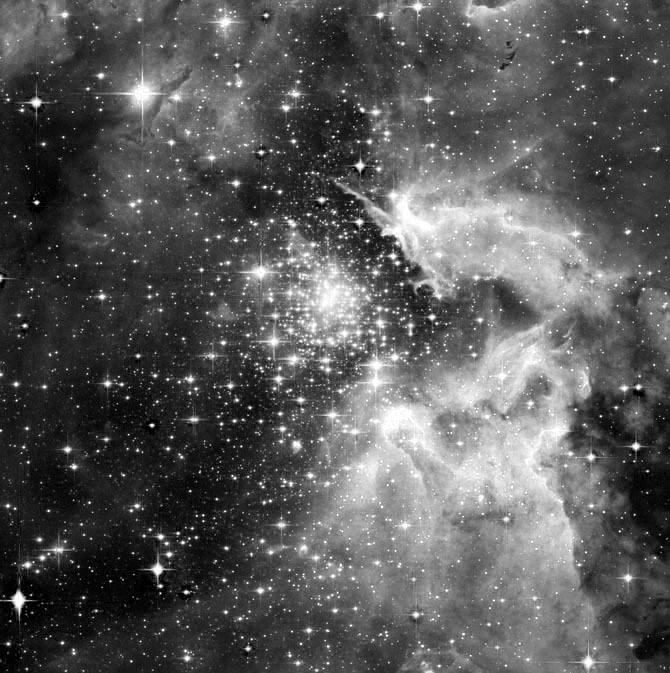
\includegraphics[scale=.2]{hubble_red.png}

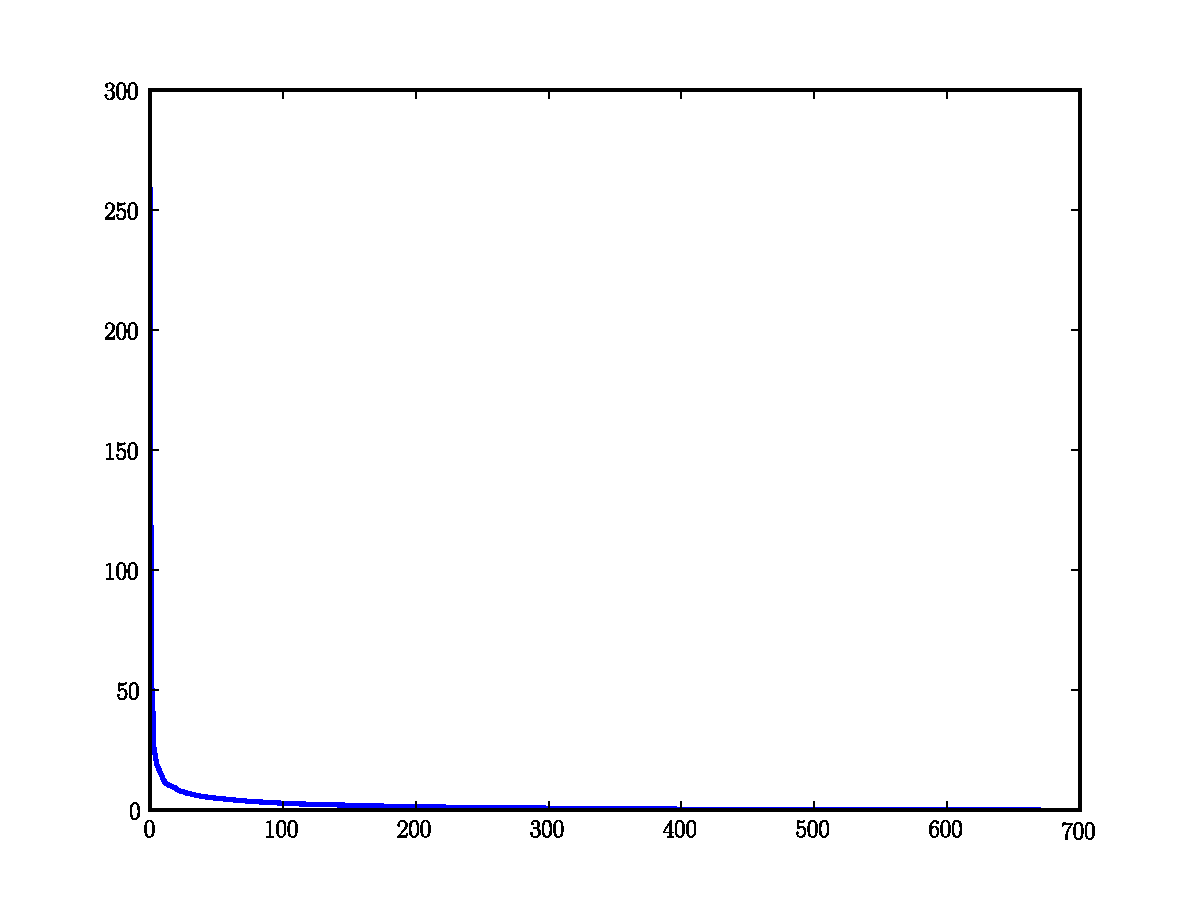
\includegraphics[scale=.4]{hubble_svals.pdf}
\end{center}

\begin{lstlisting}[style=python]
: import scipy as sp
: import numpy.linalg as nla
: A = sp.array([[1,1,3,4],[5,4,3,7],[9,10,10,12],[13,14,15,16],[17,18,19,20]])
: nla.matrix_rank(A)
: U,s,Vt = nla.svd(A)
: S = sp.diag(s)
: Ahat = sp.dot(sp.dot(U[:,0:3], S[0:3,0:3]), Vt[0:3,:])
: nla.matrix_rank(Ahat)
: nla.norm(A)-nla.norm(Ahat)
\end{lstlisting}

% We can compute the rank of a matrix by looking at the number of nonzero singular values in the SVD decompositon.  The following function will compute the rank of a matrix.  The \li{sp.finfo(float).eps} gives us the smallest representable postitive number such that $1.0+\mbox{eps} \neq 1.0$  Anything smaller than the eps value is numerically zero to the computer.
% \begin{lstlisting}[style=python]
% : def matrix_rank(X):
% :.... S = nla.svd(X, compute_uv=False)
% :.... tol = S.max()*sp.finfo(S.dtype).eps
% :.... return sum(S>tol)
% : matrix_rank(Ahat)
% \end{lstlisting}

Note that $\widehat A$ is ``close'' to the original matrix $A$, but
that its rank is 3 instead of 4.

\subsection*{Application to Imaging}


Enter the following into IPython (note that any image you might have will work):
\begin{lstlisting}
: import matplotlib.pyplot as plt
: X = sp.misc.imread('fingerprint.png')[:,:,0].astype(float)
: X.nbytes      #number of bytes needed to store X
: sp.misc.imshow(X)
\end{lstlisting}
Computing the SVD of your image is simple.  Remember to make the singluar values a diagonal matrix before multiplying.
\begin{lstlisting}
: U,s,Vt = la.svd(X)
: S = sp.diag(s)
\end{lstlisting}
In the next code block, $n$ repsents the desired rank of the output.
\begin{lstlisting}
: n=50
: u1, s1, vt1 = U[:,0:n], S[0:n,0:n], Vt[0:n,:]
: Xhat = sp.dot(sp.dot(u1, s1), vt1)
: (u1.nbytes+sp.diag(s1).nbytes+vt1.nbytes) - X.nbytes   #should be negative
: sp.misc.imshow(Xhat)
\end{lstlisting}

%write code that will caluculate final image column by column in rank 1 approximations.  It is actually smaller to transmit the matrix col by col than chunks of cols.  We only send 70% of the data if we send col by col than entire matices.  1017856bytes vs 1445888 bytes.
\begin{problem}
A law enforcement agency has been needing to efficiently store over 50,000 fingerprints.  They have decided to use an SVD based compression algorithm.  Your job is to try several parameters for the SVD algorithm and recommend those parameters that retain the highest quality but compress the most.  There should be no smearing or blocking in reconstructed final image and fingerprint detail must be retained (otherwise the fingerprint is worthless).  As part of your recommendation, calculate how much memory would be needed on average to store each compressed fingerprint.  Expand your results to say how much space could be saved if the entire database of fingerprints were compressed using your algorithm.
\end{problem}
% \begin{problem}
% Explore the clown picture for several different values of rank.
% Conduct the experiments described above.  Note that the original
% image takes 64,000 integers to store.  Compare this with the storage
% needs for various lower-rank SVD approximations. What conclusions
% can you draw? Expirement with other images we've used in this book.
% \end{problem}
